\documentclass[a4paper,11pt]{article}
\usepackage[spanish]{babel}
\usepackage[utf8]{inputenc}

\usepackage{amsmath}
\usepackage{graphicx}
\usepackage{float}
\usepackage{siunitx}


\begin{document}

\section{Introducción}

\section{Método}

	\subsection{Biblioteca utilizada}
	% Descripción biblioteca pyaudio e implementación en el código de los callbacks
	
	\subsection{Caracterización placa de sonido}
	% Respuesta en frecuencia (amplitud, fase), piso de ruido, linealidad, problemática de tirar los puntos iniciales, gráfico para describir multiplexado/demulitiplexado
	
	\begin{figure}[h]
		\centering
		\includegraphics[width=\textwidth]{imagenes/estereo.pdf}
		\caption{}
	\end{figure}
	
	
	Calibración salida: $\SI{1.62}{\V} * x + \SI{0.108}{\V}$\\
	Calibración entrada: $\SI{2.555}{\V} * x + \SI{0.09116}{\V}$\\
	
	Ruido RMS = \SI{277}{\uV}.
	
	\begin{figure}[h]
		\centering
		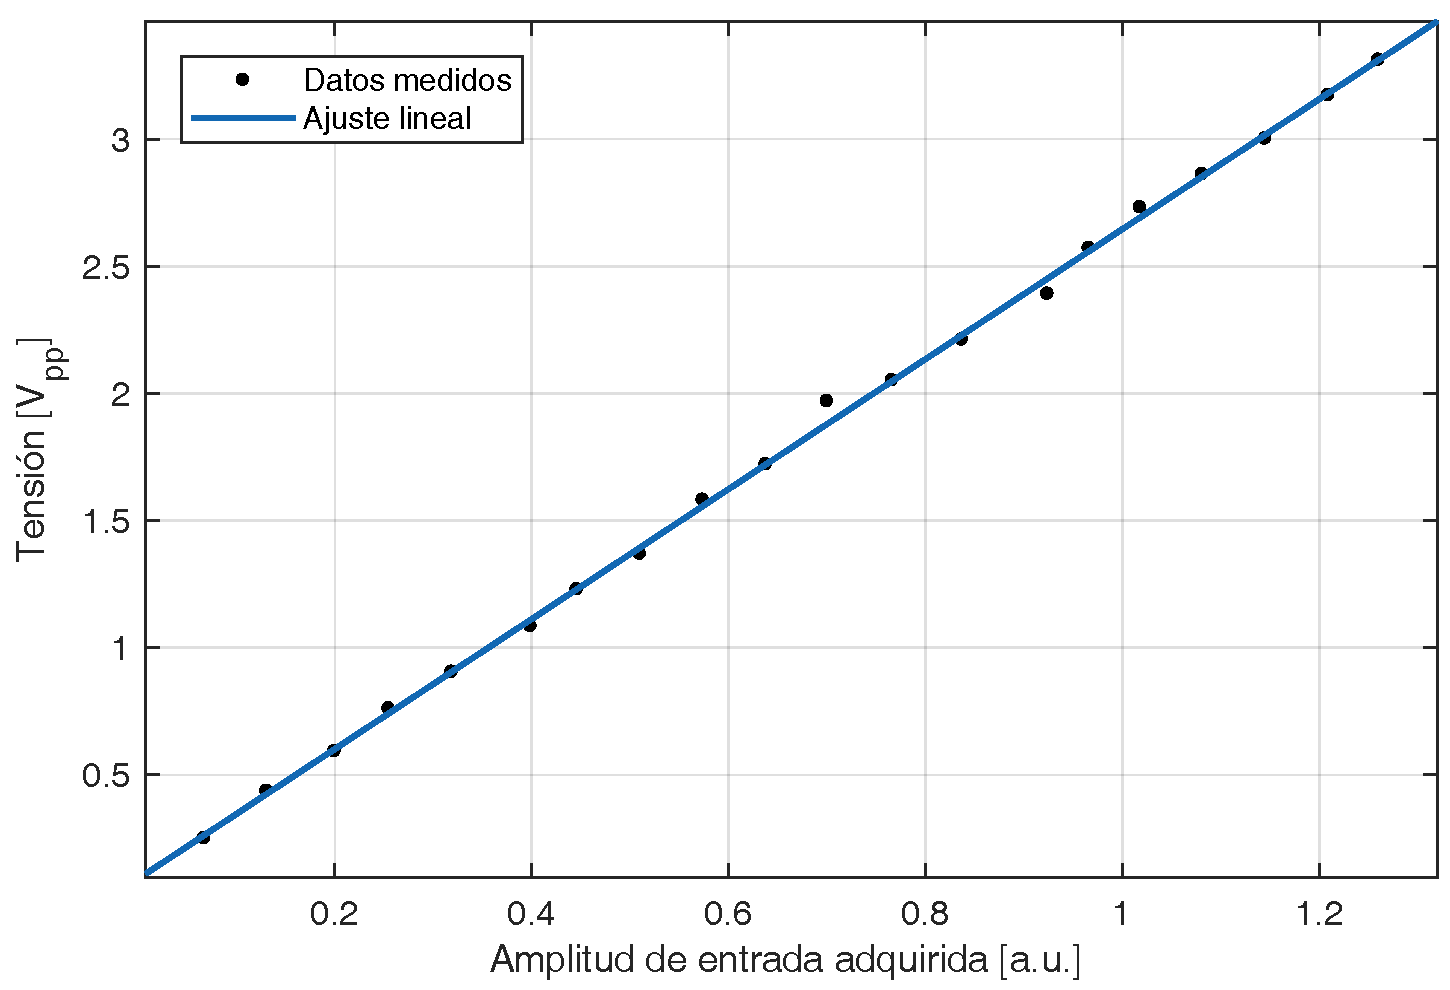
\includegraphics[width=\textwidth]{imagenes/CalibracionEntrada.pdf}
		\caption{}
	\end{figure}
	
	\begin{figure}[h]
		\centering
		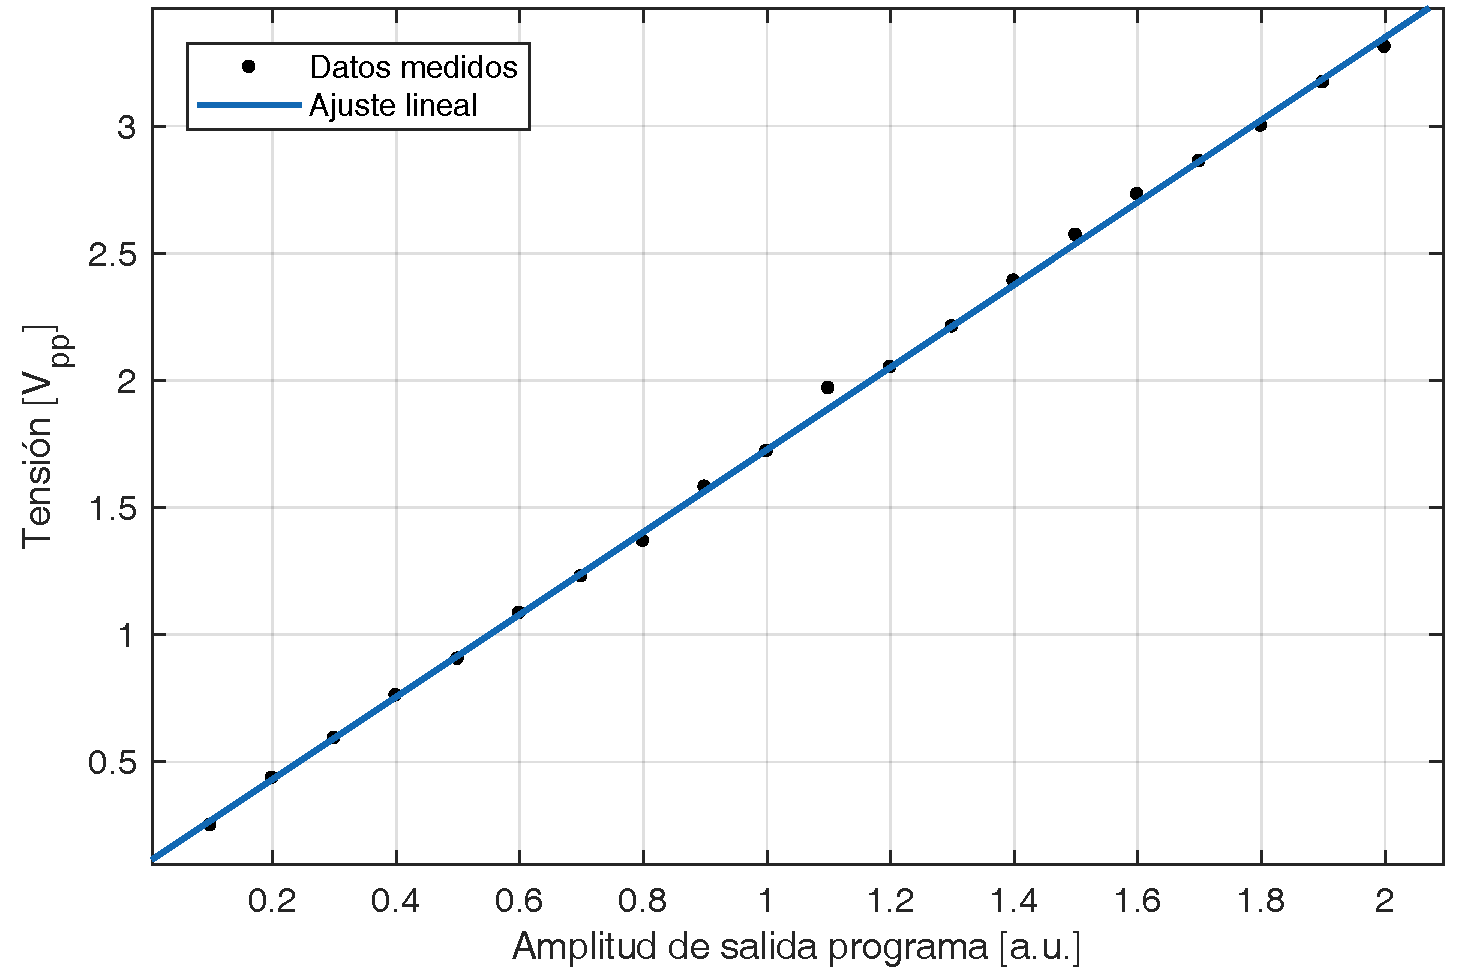
\includegraphics[width=\textwidth]{imagenes/CalibracionSalida.pdf}
		\caption{}
	\end{figure}
	
	\begin{figure}[h]
		\centering
		\includegraphics[width=\textwidth]{imagenes/bode44k1Hz.png}
		\caption{}
	\end{figure}

	\begin{figure}[h]
		\centering
		\includegraphics[width=\textwidth]{imagenes/bode192kHz.png}
		\caption{}
	\end{figure}
	
	\begin{figure}[h]
		\centering
		\includegraphics[width=\textwidth]{imagenes/RuidoCanalIzquierdo.png}
		\caption{}
	\end{figure}
	
	\begin{figure}[h]
		\centering
		\includegraphics[width=\textwidth]{imagenes/RuidoCanalDerecho.png}
		\caption{}
	\end{figure}

\section{Resultados}

	\subsection{Discreto}
	% Curva I-V
	
	\begin{figure}[h]
		\centering
		\includegraphics[width=\textwidth]{imagenes/Diodo1N4148.png}
		\caption{}
	\end{figure}
	
	\subsection{Integrado}
	

\end{document}